\documentclass[tikz,border=2pt]{standalone}
\usetikzlibrary{arrows.meta,positioning,fit,calc,shapes.geometric,decorations.pathmorphing}
\definecolor{blueMain}{HTML}{0B4E94}
\definecolor{blueSoft}{HTML}{EAF2FA}
\definecolor{tealMain}{HTML}{3B9AA3}
\definecolor{greenSoft}{HTML}{DDF3DE}
\definecolor{redMain}{HTML}{B64342}
\definecolor{redSoft}{HTML}{F6CFCB}
\definecolor{goldMain}{HTML}{D99A21}
\definecolor{goldSoft}{HTML}{FFF2CC}
\definecolor{violetMain}{HTML}{6B3FB4}
\definecolor{violetSoft}{HTML}{F4ECFF}
\definecolor{greyText}{HTML}{222222}
\definecolor{greyLine}{HTML}{8D8D8D}
\definecolor{panel}{HTML}{F8F8F8}
\tikzset{
  blk/.style={draw=#1, rounded corners=2pt, thick, align=center, fill=white,
    inner sep=2.4pt, font=\sffamily\scriptsize},
  dashedblk/.style={draw=#1, dashed, rounded corners=2pt, thick, align=center,
    fill=white, inner sep=2.4pt, font=\sffamily\scriptsize},
  arr/.style={-{Stealth[length=2mm]}, thick},
  arrblue/.style={-{Stealth[length=2mm]}, very thick, blueMain},
  num/.style={circle, draw=blueMain, text=blueMain, fill=white, inner sep=0.45pt,
    minimum size=0.23cm, font=\sffamily\tiny\bfseries},
  tinytext/.style={font=\sffamily\tiny, align=center},
  dot/.style={circle, fill=greyLine, inner sep=1pt}
}
\newcommand{\Step}[3]{\node[num] at (#1,#2) {#3};}
\newcommand{\Cylinder}[3]{%
  \draw[#3, thick, fill=#2] (#1) ellipse (0.18 and 0.06);
  \draw[#3, thick, fill=#2] ($(#1)+(-0.18,0)$) -- ++(0,-0.34) arc[start angle=180,end angle=360,x radius=0.18,y radius=0.06] -- ++(0,0.34);
}
\newcommand{\NetIcon}[3]{%
  \foreach \p in {(#1,#2),(#1+0.34,#2+0.17),(#1+0.34,#2-0.17),(#1+0.68,#2)}
    \node[circle, draw=#3, fill=white, inner sep=1.2pt] at \p {};
  \draw[#3, thick] (#1,#2) -- (#1+0.34,#2+0.17) -- (#1+0.68,#2) -- (#1+0.34,#2-0.17) -- cycle;
}
\begin{document}
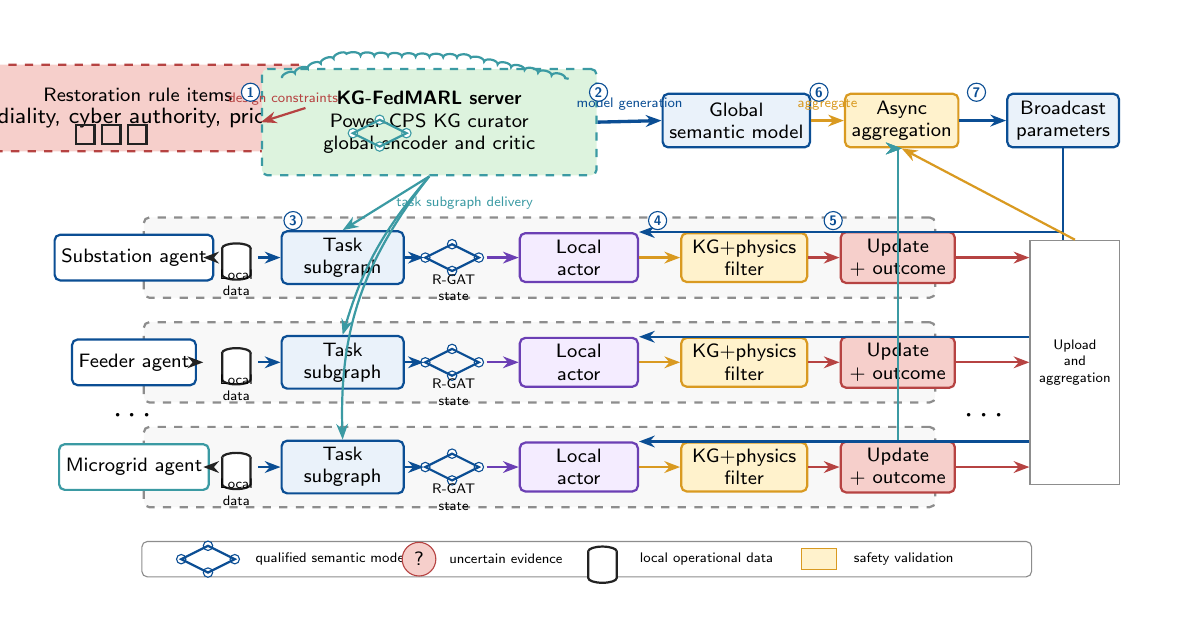
\begin{tikzpicture}[x=1cm,y=1cm,font=\sffamily\scriptsize]
  \path[use as bounding box] (0.05,0.05) rectangle (14.50,7.30);

  % Left rule/contract block similar to template contract items.
  \node[dashedblk=redMain, fill=redSoft, minimum width=2.40cm, minimum height=1.10cm] (rules) at (1.45,6.28)
    {Restoration rule items\\\footnotesize radiality, cyber authority, priority};
  \draw[greyText, thick] (0.66,5.82) rectangle (0.90,6.06);
  \draw[greyText, thick] (0.99,5.82) rectangle (1.23,6.06);
  \draw[greyText, thick] (1.32,5.82) rectangle (1.56,6.06);

  % Curator / KG server.
  \node[dashedblk=tealMain, fill=greenSoft, minimum width=4.25cm, minimum height=1.35cm] (curator) at (5.15,6.10)
    {\textbf{KG-FedMARL server}\\Power-CPS KG curator\\global encoder and critic};
  \draw[tealMain, thick, decorate, decoration={bumps,segment length=0.35cm,amplitude=1.2pt}]
    (3.28,6.66) -- (4.05,6.95) -- (5.60,6.92) -- (6.92,6.65);
  \NetIcon{4.18}{5.96}{tealMain}
  \node[blk=blueMain, fill=blueSoft, minimum width=1.38cm, minimum height=0.68cm] (global) at (9.05,6.12)
    {Global\\semantic model};
  \node[blk=goldMain, fill=goldSoft, minimum width=1.30cm, minimum height=0.68cm] (agg) at (11.15,6.12)
    {Async\\aggregation};
  \node[blk=blueMain, fill=blueSoft, minimum width=1.42cm, minimum height=0.68cm] (bcast) at (13.20,6.12)
    {Broadcast\\parameters};

  \draw[arr, redMain] (rules.east) -- node[above,tinytext] {design constraints} (curator.west);
  \draw[arrblue] (curator.east) -- node[above,tinytext] {model generation} (global.west);
  \draw[arr, goldMain] (global.east) -- node[above,tinytext] {aggregate} (agg.west);
  \draw[arrblue] (agg.east) -- (bcast.west);
  \Step{2.88}{6.48}{1}
  \Step{7.30}{6.48}{2}
  \Step{10.10}{6.48}{6}
  \Step{12.10}{6.48}{7}

  % Data owner / agent rows.
  \foreach \y/\name/\icon/\clr in {4.38/Substation agent/S/blueMain,3.05/Feeder agent/F/blueMain,1.72/Microgrid agent/M/tealMain} {
    \node[dashedblk=greyLine, fill=panel, minimum width=10.05cm, minimum height=1.02cm] (row\icon) at (6.55,\y) {};
    \node[blk=\clr, fill=white, minimum width=1.08cm, minimum height=0.58cm] (do\icon) at (1.40,\y) {\name};
    \Cylinder{2.70,\y+0.12}{white}{greyText}
    \node[tinytext] at (2.70,\y-0.32) {Local\\data};
    \node[blk=blueMain, fill=blueSoft, minimum width=1.55cm, minimum height=0.58cm] (q\icon) at (4.05,\y) {Task\\subgraph};
    \NetIcon{5.10}{\y}{blueMain}
    \node[tinytext] at (5.46,\y-0.38) {R-GAT\\state};
    \node[blk=violetMain, fill=violetSoft, minimum width=1.50cm, minimum height=0.58cm] (actor\icon) at (7.05,\y) {Local\\actor};
    \node[blk=goldMain, fill=goldSoft, minimum width=1.60cm, minimum height=0.58cm] (safe\icon) at (9.15,\y) {KG+physics\\filter};
    \node[blk=redMain, fill=redSoft, minimum width=1.45cm, minimum height=0.58cm] (up\icon) at (11.10,\y) {Update\\+ outcome};
    \draw[arr, greyText] (do\icon.east) -- (2.28,\y);
    \draw[arr, blueMain] (2.98,\y) -- (q\icon.west);
    \draw[arr, blueMain] (q\icon.east) -- (5.08,\y);
    \draw[arr, violetMain] (5.88,\y) -- (actor\icon.west);
    \draw[arr, goldMain] (actor\icon.east) -- (safe\icon.west);
    \draw[arr, redMain] (safe\icon.east) -- (up\icon.west);
    \draw[arr, blueMain] (bcast.south) |- (actor\icon.north east);
    \draw[arr, tealMain] (up\icon.north) |- (agg.south);
  }
  \node[font=\sffamily\large] at (1.38,2.37) {$\cdots$};
  \node[font=\sffamily\large] at (12.20,2.37) {$\cdots$};

  % Step labels and arrows from server to clients.
  \draw[arr, tealMain] (curator.south) -- node[right,tinytext] {task subgraph delivery} (qS.north);
  \draw[arr, tealMain] (curator.south) to[bend right=12] (qF.north);
  \draw[arr, tealMain] (curator.south) to[bend right=20] (qM.north);
  \Step{3.42}{4.85}{3}
  \Step{8.05}{4.85}{4}
  \Step{10.28}{4.85}{5}

  % Side feedback/aggregation bar to mimic template vertical aggregation channel.
  \node[draw=greyLine, fill=white, minimum width=0.45cm, minimum height=3.10cm, align=center,
    font=\sffamily\tiny] (bar) at (13.35,3.05) {Upload\\and\\aggregation};
  \draw[arr, redMain] (upS.east) -- (bar.west |- upS.east);
  \draw[arr, redMain] (upF.east) -- (bar.west |- upF.east);
  \draw[arr, redMain] (upM.east) -- (bar.west |- upM.east);
  \draw[arr, goldMain] (bar.north) -- (agg.south);

  % Legend strip, template-like.
  \node[draw=greyLine, fill=white, rounded corners=2pt, minimum width=11.30cm, minimum height=0.45cm] at (7.15,0.55) {};
  \NetIcon{2.00}{0.55}{blueMain}
  \node[tinytext, anchor=west] at (2.82,0.55) {qualified semantic model};
  \node[circle, draw=redMain, fill=redSoft, inner sep=2.2pt] at (5.02,0.55) {?};
  \node[tinytext, anchor=west] at (5.28,0.55) {uncertain evidence};
  \Cylinder{7.35,0.65}{white}{greyText}
  \node[tinytext, anchor=west] at (7.70,0.55) {local operational data};
  \node[draw=goldMain, fill=goldSoft, minimum width=0.45cm, minimum height=0.26cm] at (10.10,0.55) {};
  \node[tinytext, anchor=west] at (10.42,0.55) {safety validation};
\end{tikzpicture}
\end{document}
